
\documentclass[12pt]{article}
\setlength\parindent{0pt}
\usepackage{fullpage}
\usepackage{amsmath}
\usepackage{graphicx}
\setlength{\parskip}{4mm}
\def\LL{\left\langle}   % left angle bracket
\def\RR{\right\rangle}  % right angle bracket
\def\LP{\left(}         % left parenthesis
\def\RP{\right)}        % right parenthesis
\def\LB{\left\{}        % left curly bracket
\def\RB{\right\}}       % right curly bracket
\def\PAR#1#2{ {{\partial #1}\over{\partial #2}} }
\def\PARTWO#1#2{ {{\partial^2 #1}\over{\partial #2}^2} }
\def\PARTWOMIX#1#2#3{ {{\partial^2 #1}\over{\partial #2 \partial #3}} }
\newcommand{\BE}{\begin{displaymath}}
\newcommand{\EE}{\end{displaymath}}
\newcommand{\BNE}{\begin{equation}}
\newcommand{\ENE}{\end{equation}}
\newcommand{\BEA}{\begin{eqnarray}}
\newcommand{\EEA}{\nonumber\end{eqnarray}}
\newcommand{\EL}{\nonumber\\}
\newcommand{\la}[1]{\label{#1}}
\newcommand{\ie}{{\em i.e.\ }}
\newcommand{\eg}{{\em e.\,g.\ }}
\newcommand{\cf}{cf.\ }
\newcommand{\etc}{etc.\ }
\newcommand{\Tr}{{\rm tr}}
\newcommand{\etal}{{\it et al.}}
\newcommand{\OL}[1]{\overline{#1}\ } % overline
\newcommand{\OLL}[1]{\overline{\overline{#1}}\ } % double overline
\newcommand{\OON}{\frac{1}{N}} % "one over N"
\newcommand{\OOX}[1]{\frac{1}{#1}} % "one over X"



\begin{document}
\Large
\centerline{\sc{Recitation Questions}}
\normalsize
\centerline{\sc{April 5}}

\begin{enumerate}
\item If you didn't have time to complete this problem last week, complete it.

\begin{minipage}[b]{0.4\textwidth}
  \vspace{-2.8in}

A 4m-long pole of mass 80 kg extends from the side of a building, angled at 60 degrees above the horizontal. One meter from the end of the pole, a sign of mass 50 kg is attached. To support the pole,
a horizontal cable runs from the end of the pole to the building. (See the attached figure.)

\bigskip
\bigskip
\bigskip
\bigskip
\bigskip
\bigskip

\end{minipage}
\begin{minipage}[t]{0.6\textwidth}
  \begin{flushright}
  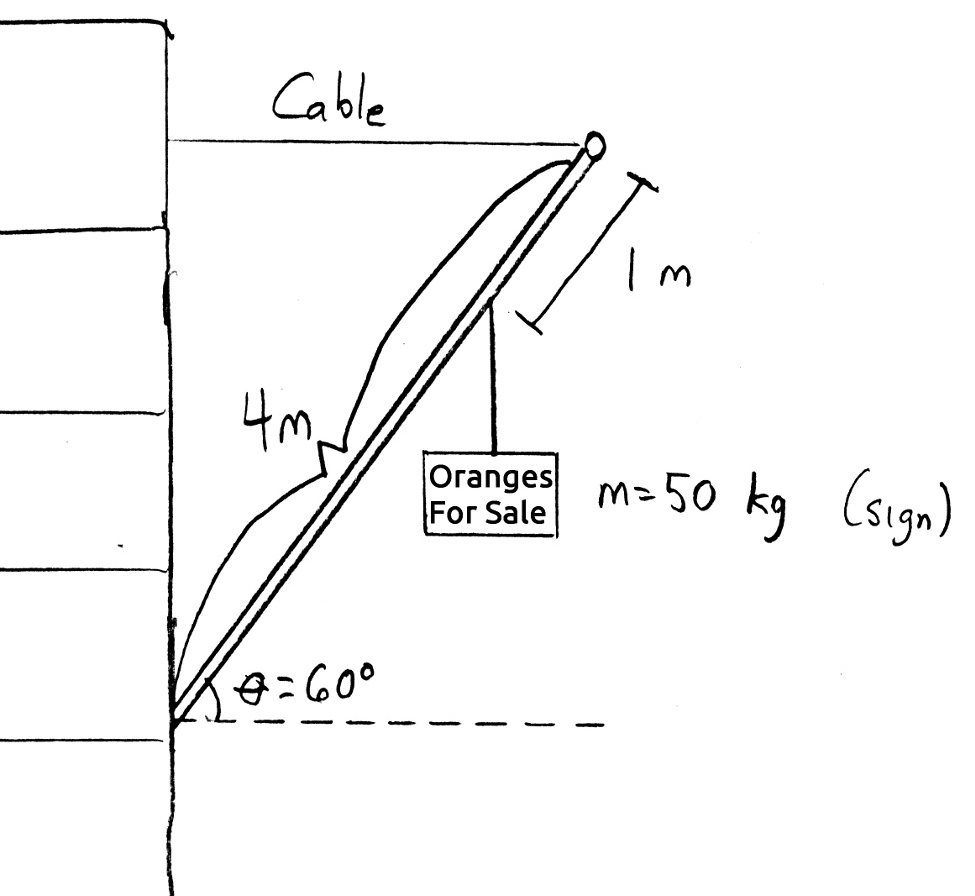
\includegraphics[width=0.9\textwidth]{sign2.jpg}
\end{flushright}
\end{minipage}

\bigskip
\bigskip

\begin{enumerate}
\item Draw a force diagram on the back of this page, showing all of the elements needed to help you compute the tension in the support cable. Indicate
your choice of pivot point.

\bigskip

\item Compute the tension in the cable.

\vspace{2 in}

\item Suppose now that the store owner wanted to attach the cable to a different point on the building in order to minimize its tension. What angle between the
cable and the horizontal would support the pole with the minimum tension?
\end{enumerate}
\newpage


  \item{A light cable is wound around a cylindrical spool fixed in place of radius 50 cm and mass 10 kg. One end of the cable is attached to a motor, which pulls with a constant force of 20 N on the cable. When the motor is switched on, the force exerted by the cable causes the spool to rotate faster and faster.}
    \begin{enumerate}
      \item{What is the moment of inertia of the spool?}
\vspace{0.9in}
      \item{What is the torque applied to the spool by the motor?}
\vspace{0.9in}
      \item{What is the angular acceleration of the spool?}
\vspace{0.9in}
      \item{How long will it take for the spool to make a full revolution?}
\vspace{0.9in}
      \item{After five seconds, how fast is the cable moving?}
\vspace{0.9in}
      \item{After five seconds, what is the kinetic energy of the spool? Remember that the kinetic energy
of a rotating object is $\frac{1}{2}I\omega^2$.}
\vspace{0.9in}
      \item{What is the work done by the motor in five seconds? Remember that the rotational work-energy
theorem is $W=\tau \Delta \theta$.}
\vspace{0.9in}
     \end{enumerate}

\newpage

\item A flywheel (a large, spinning disc) of mass $m$ and radius $r$ is rotating
at angular velocity $\omega$. The machine operator wishes to bring it to rest using a brake. When the brake 
is engaged, two brake pads on either side of the disc are pressed against it from either side, two-thirds
of the way from the center to the outer edge; each brake pad
exerts a normal force $F_N$. 

If the coefficient of friction between the brake pads and the disc is $\mu_k$, how long does it take the
brake to bring the flywheel to a stop?


     \end{enumerate}

\newpage
\centerline{\sc{Reference Material - Rotational Motion}}


Moments of Inertia:
\begin{itemize}
  \item{Disk or cylinder, rotating about center: $I = \frac{1}{2}MR^2$}
  \item{Sphere, rotating about center: $I = \frac{2}{5}MR^2$}
  \item{Ring or hollow cylinder, rotating about center: $I = MR^2$}
\end{itemize}

\bigskip
\bigskip
\bigskip

Correspondence between linear dynamics and rotational dynamics: 
  \scriptsize

\begin{tabular}{| c | c | c | c |}
  \hline
  Position & $s$ & Angle & $\theta$  \\
  Velocity & $\vec v$ & Angular velocity & $\omega$  \\
  Acceleration & $\vec a$ & Angular acceleration & $\alpha$  \\
  \hline
                                   & $v(t) = v_0 + at$ & & $\omega(t) = \omega_0 + \alpha t$ \\
                                   & $x(t) = x_0 + v_0 t + \frac{1}{2} at^2$ & & $\theta(t) = \theta_0 + \omega_0 t + \frac{1}{2} \alpha t^2$ \\
                                   & $v_f^2 - v_0^2 = 2a \Delta x$ & & $\omega_f^2 - \omega_0^2 = 2 \alpha \Delta \theta$ \\
  \hline
  Mass & $m$ & Moment of inertia & $I$ \\
  \hline
  Force & $F$ & Torque & $\tau = F_\perp r = F r_\perp$ \\
  \hline
  Newton's second law & $\vec F = m \vec a$ & ``Newton's second law for rotation'' & $\tau = I \alpha$ \\
  \hline
  Kinetic energy & $\frac{1}{2} mv^2$ & Kinetic energy & $\frac{1}{2}I\omega^2$ \\
  \hline
  Momentum & $\vec p = m \vec v$ & Angular momentum & $L = I \omega$ \\
  \hline
\end{tabular}

\bigskip
\bigskip
\bigskip

Arc length $s=\theta r$ \\
Tangential velocity $v=\omega r$ \\
Tangential acceleration $a=\alpha r$




 \end{document}
